%
% ------------------------------------------------------------------------------
\section{The Earthquake Rupture Forecast Calculator}
\index{Seismic Sources!Model}
\index{Seismic Sources!Initial Model}
The \gls{earthquakeruptureforecast} is a fundamental concept in the OpenSHA 
framework \citep{field2003} as well as in the hazard component of OpenQuake.

As explained in the previous Section, the calculation of the \gls{acr:erf} 
in OQ starts from a \gls{seismicsourcemodel} created by the  
\gls{logictreeprocessor}.
%
When epistemic uncertainty is not included in the seismic source 
system there exists a one to one correspondance between the 
\gls{initialseismicsourcemodel} and the \gls{seismicsourcemodel} used 
in the calculation of hazard. In this case, the \gls{logictreeprocessor} 
just duplicates into the \gls{seismicsourcemodel} the information 
included in the \gls{initialseismicsourcemodel}.
%
In more complicated cases, when epistemic uncertainty affects many 
parameters characterizing seismic sources, the \gls{logictreeprocessor} 
generates many \glspl{acr:ssm} so as to explore entirely the space 
of models admitted by our imprecise knowledge.

Independently of the complication of the seismic source logic tree,
the Earthquake Rupture Forecast calculator processes one at a time the 
\glspl{acr:ssm} and creates a list of the ruptures generated by all 
the sources included. 
%
Each rupture in the list is associated with a probability of occurrence 
in the \gls{investigationtime} specified by the user in the calculation 
settings. To produce this results, the earthquake rupture forecast 
calculator treats separately each source typology included in the 
seismic source model. A detailed description of the methodologies 
adopted to create the earthquake rupture forecast for different seismic
source types is provided in the following Sections.

As a final important note: for the time being - OQ supports just sources 
producing seismicity in accordance with a Possion temporal occurrence model.
%
% - - - - - - - - - - - - - - - - - - - - - - - - - - - - - - - - - - - -- - - -
\subsection{ERF creation in case of distributed seismicity}
Open Quake supports two seismic source typologies capable to model 
distributed seismicity: \glspl{areasource} and \glspl{gridsource}.

Area sources are the most traditional source type adopted in PSHA 
analysis since its first introduction at the end of the 1960s. 
%
The works of \cite{frankel1995} and \cite{frankel1997} boosted the 
use of grid sources in probabilistic seismic hazard calculations. 
%
%. . . . . . . . . . . . . . . . . . . . . . . . . . . . . . . . . . . . . . . .
\subsubsection{Area source}
%
The creation of an ERF in case of \glspl{areasource} (see also Section 
\ref{hazard:seismic_source_types:areaSources} at page 
\pageref{hazard:seismic_source_types:areaSources}) requires a 
preliminary step consisting in the discretization of the polygon 
used to delimit the spatial extension of the source. 
%
% . . . . . . . . . . . . . . . . . . . . . . . . . . . . . . . . . . . > Figure
\begin{figure}[!ht]
\centering
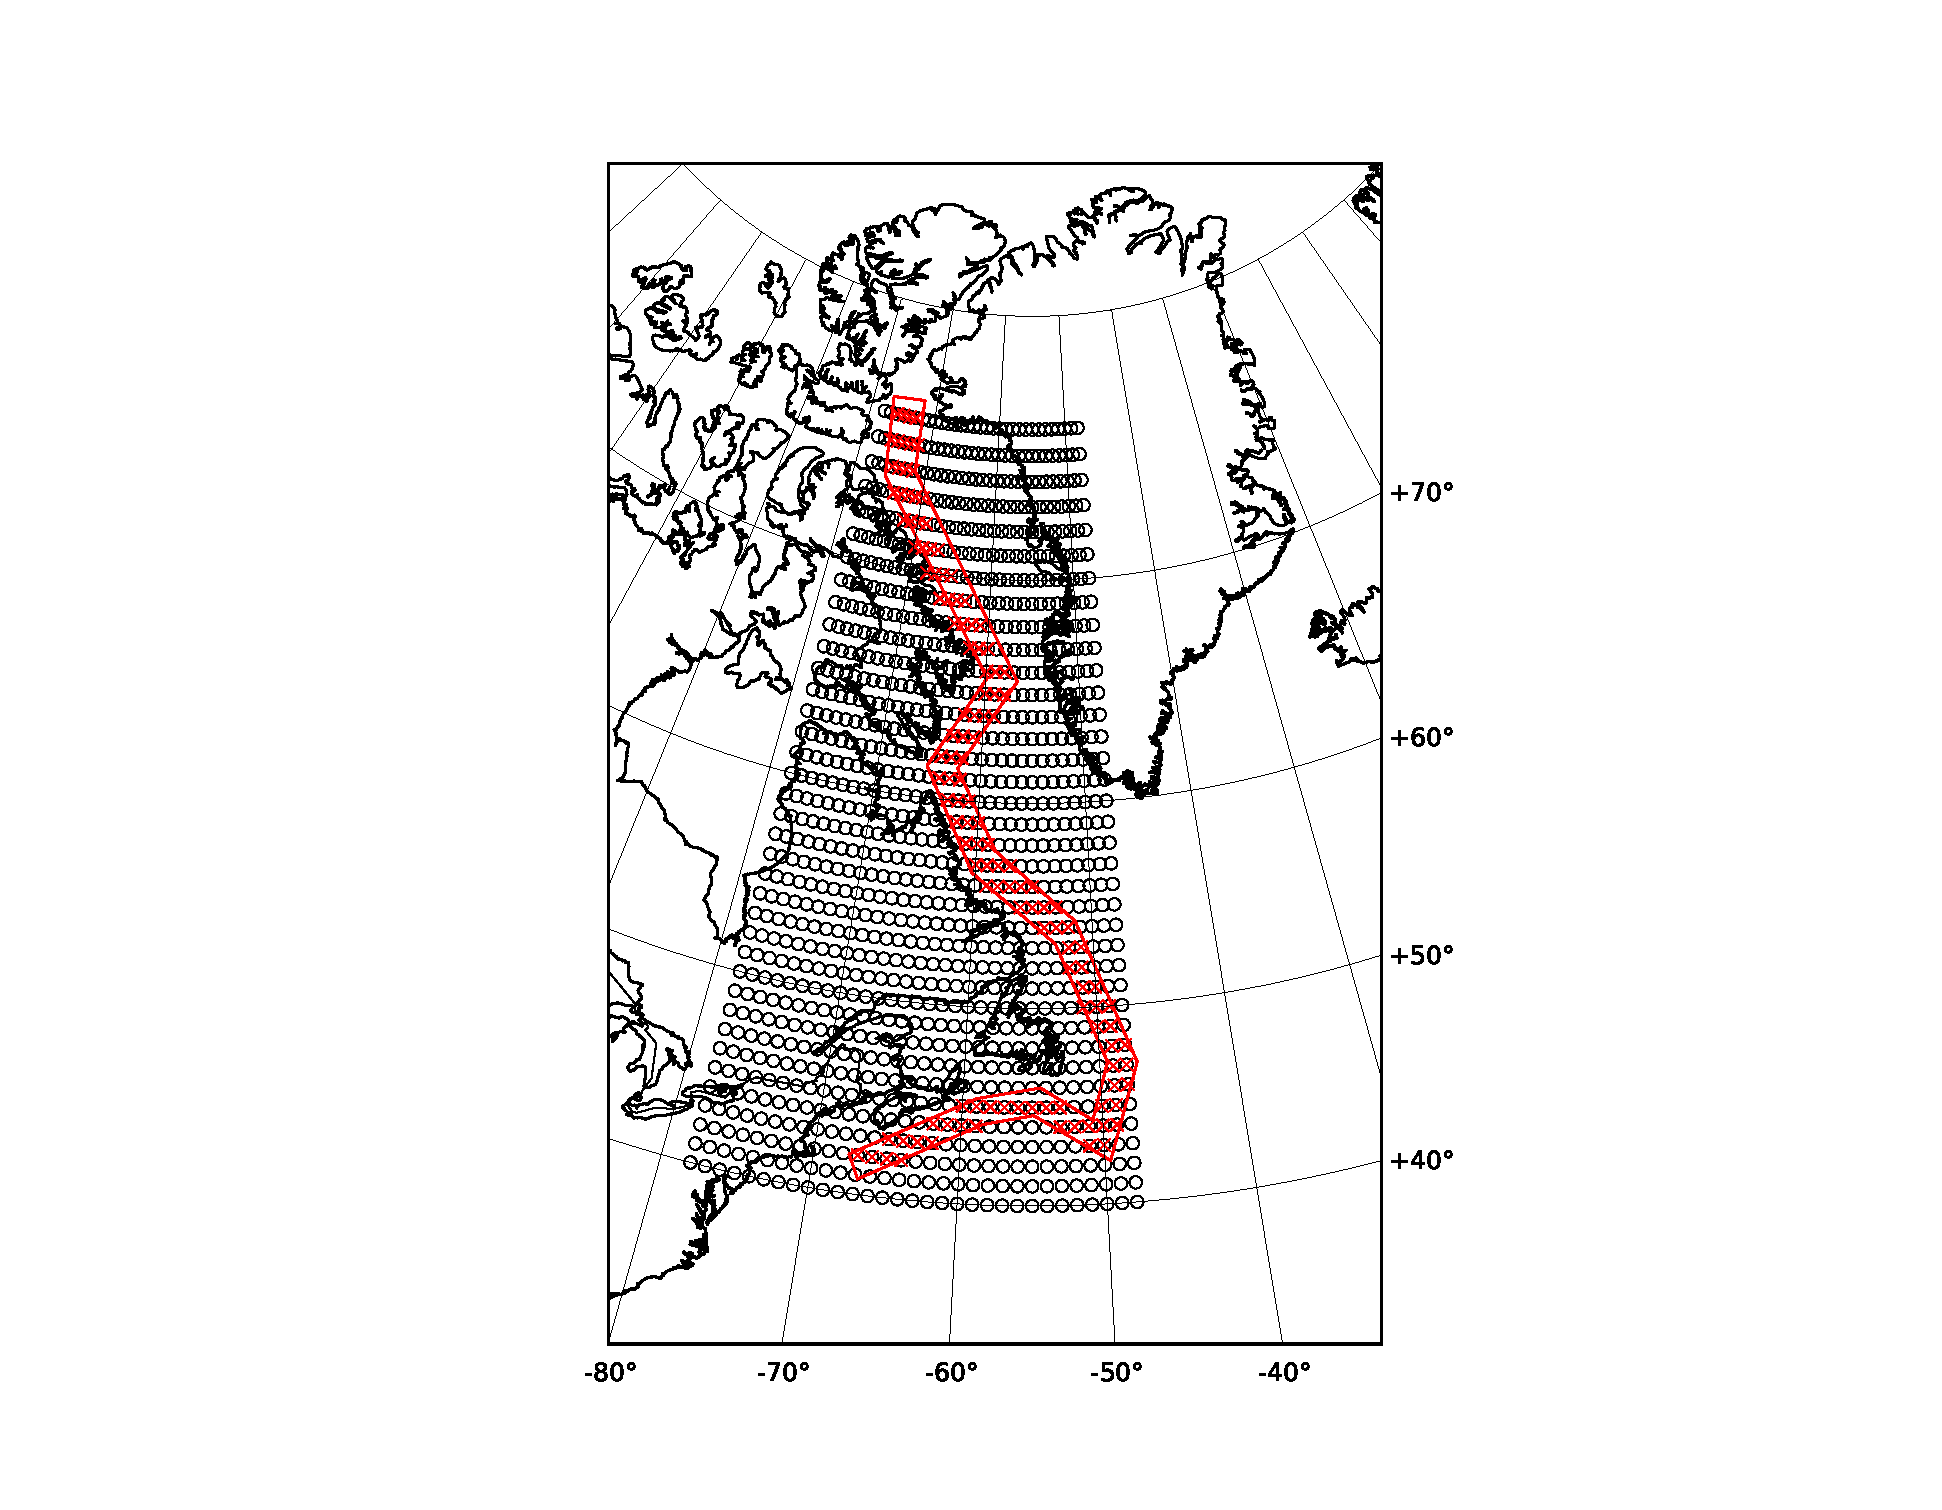
\includegraphics[width=18cm]{./Figures/Part_Hazard/area_source_discretization.eps}
\caption{Example of an area source discretisation (grid spacing equal 
to 0.5$^\circ$). Note how the spacing between circles decreases moving from 
bottom to top of the source.}
\label{fig:area_source_discret}
\end{figure}
% . . . . . . . . . . . . . . . . . . . . . . . . . . . . . . . . . . . < Figure
%
OQ discretizes area sources by overlapping a regular grid of nodes
over the polygon representing the source. The grid contains nodes 
equally spaced in latitude and longitude; the position of each node
is specified by one geographic coordinate, expressed in decimal degrees. 
The nodes of the grid inside the polygon represent - in a discrete way - 
the area source.

The reference system adopted has the advantage that is simple and 
intuitive, however from a computational point of view it has some 
drawback. The most relevant one is that the spacing (in km) between 
nodes of the grid depends on latitude. 
%
Indeed, the spacing of between two nearby nodes near the equator is 
larger than at high latitudes e.g. one degree of longitude at the equator 
correponds to about 111 km, at 45$^\circ$ of latitude it becomes 
about 78.8 km and, at 75$^\circ$ it corresponds to only 28 km. 
%
Figure \ref{fig:area_source_discret} shows a discretization example 
considering an area source contained in the Canada model. If we assume 
the grid nodes as centers of rectangular cells, the shape of these cells
tends to be squeezed as we move towards the poles.

The problem of this uneven distribution of cell size arises when we 
distribute the seismicity defined for the entire area source over the 
nodes used to represent its shape. If the node spacing was homogenous,
the seismicity on each node would be simply the total seismicity divided 
by the number of nodes selected to discretize the area source.
%
In reality this condition is never satisfied, as a consequence, to 
guarantee an homogeneous distribution of seismicity rates \gls{acr:oq} 
we adopt a simple procedure that distributes the seismicity rates 
proportionally to the cell size (i.e grid node spacing).
%
Particularly, for each node of an area source we compute the area using
the following relationship:
\begin{equation}
 \text{area} = 4\pi^2 * \text{grid\_spacing}^2 *  
 	\left(\frac{\text{earth\_radius}}{360}\right)^2 * 
 	\sin(\text{node\_latitude})
 	\label{eq:cell_area}
\end{equation}
where:
\begin{itemize}
\item grid\_spacing is the distance between two consecutive cells 
	of the grid adopted to discretize the area source (a common value 
	adopted to discretize sources is equal to 0.1)
\item earth\_radius is the mean radius of the Earth (approximately 
	6371 km) 
\item node\_latitude is the latitude of the cell of which we compute
	the area.
\end{itemize}
%
To get the seismicity rates for a single grid node we multiply the 
ratio between the area (computed using equation \ref{eq:cell_area}) and 
the area of the entire source (i.e. the sum of the areas computed 
with looping for the grid nodes used to discretize the source polygon).
%
%. . . . . . . . . . . . . . . . . . . . . . . . . . . . . . . . . . . . . . . .
\subsubsection{Multi-depth area source}
%
This source typology is an extension of the just described area source, 
it allows to distribute seismicity within a volume delimited by the 
projection of a polygon lying on the topographic surface along the 
depth-axis and two planes parallel to the topographic surface 
identifying the upper and lower seismogenic depth.

The creation of the \gls{acr:erf} in case of multi-depth area sources
follows the same criteria discussed in the previous section for area
sources. The \gls{acr:fmd} for the entire source is distributed over 
the nodes of the 3D grid used to describe the multi-depth volume.
%
%. . . . . . . . . . . . . . . . . . . . . . . . . . . . . . . . . . . . . . . .
\subsubsection{Grid source}
\Glspl{gridsource} are a source typology that's becoming a valuable alternative
to area sources when modeling distributed seismicity. 
%
The main advantage of grid sources consists on the seismicity smoothing 
procedure that's laying behind their calculation. Seismicity smoothing 
indeed is an objective methodology, reproducible and - usually - not
particularly complex. 

The creation of the ERF in case of \glspl{gridsource} follows the same 
concepts described in the previous section in case of area sources. 
%
The main difference is that with this source type the discretisation step 
is not needed.

%- - - - - - - - - - - - - - - - - - - - - - - - - - - - - - - - - - - - - - - -
\subsubsection{Accounting for rupture finiteness in case of distributed 
seismicity}
%
Each node used to discretise an area source or a multi-depth area 
source or belonging to a grid source has tuples composed by 
the following objects:
\begin{itemize}
\item A discrete representation of a \gls{acr:fmd} 
\item A faulting style, that is strike [optional], dip [optional] and 
rake [optional] 
\end{itemize}
The definition of one, or several, faulting styles is optional; this 
means that in the simplest case only one discrete FMD is specified.

%The \gls{earthquakeruptureforecastcalculator} operates in agreement with
%the parameters specifying the properties of each single node composing
%a seismic source:
%\begin{enumerate}
%\item If no faulting style parameters are specified:
%	\begin{enumerate}
%	\item If the finiteness of the ruptures has to be considered in the 
%	calculation (at least for a given specific magnitude range)
%	\end{enumerate}
%\item If only strike is specified:
%	\begin{enumerate}
%	\item If the finiteness of the ruptures has to be considered in the 
%	calculation (at least for a given specific magnitude range)
%	\end{enumerate}
%\item If strike and rake are specified:
%	\begin{enumerate}
%	\item If the finiteness of the ruptures has to be considered in the 
%	calculation (at least for a given specific magnitude range)
%	\end{enumerate}
%\item If strike, dip and rake are specified:
%	\begin{enumerate}
%	\item If the finiteness of the ruptures has to be considered in the 
%	calculation (at least for a given specific magnitude range)
%	\end{enumerate}
%\item
%\end{enumerate}
%%

% - - - - - - - - - - - - - - - - - - - - - - - - - - - - - - - - - - - - - - - 
\clearpage
\subsection{ERF creation in case of Fault sources}

%
%. . . . . . . . . . . . . . . . . . . . . . . . . . . . . . . . . . . . . . . .
\subsubsection{Fault sources with simple geometry}
Simple faults in OQ are representations of tectonic structures with a . 
The methodology adopted fot the creation of the fault surface uses the 
fault trace, a representative dip direction (e.g. it could be the mean 
dip direction) and, the upper and lower seismogenic depth. 

%
%. . . . . . . . . . . . . . . . . . . . . . . . . . . . . . . . . . . . . . . .
\subsubsection{Fault sources with complex geometry}

%
%. . . . . . . . . . . . . . . . . . . . . . . . . . . . . . . . . . . . . . . .
\subsubsection{Computing the probability of occurrence of each rupture}
In OQ, by convention, we describe the frequency-magnitude distribution using 
a discrete representation. 
This choice offers the largest flexibility in describing the rate of 
earthquakes with respect to magnitude. 
%
% . . . . . . . . . . . . . . . . . . . . . . . . . . . . . . . . . . . > Figure
\begin{figure}[!ht]
\includegraphics[width=15cm]{./Figures/Part_Hazard/gr_example.eps}
\caption{Example of a discrete incremental frequency-magnitude Gutenberg-Richter distribution}
\label{fig:gr-example}
\end{figure}
% . . . . . . . . . . . . . . . . . . . . . . . . . . . . . . . . . . . < Figure
%

